\documentclass{superfri}

\usepackage{amsfonts}
\usepackage{amssymb}
\usepackage[cmex10]{amsmath}
\usepackage{booktabs}
\usepackage{enumitem}
\usepackage{graphicx}
\usepackage{fancyvrb}
\usepackage{ifthen}
\usepackage{cite}
\usepackage{tabulary}
\usepackage{url}
\usepackage{xspace}
\usepackage{wrapfig}
\usepackage[pdfborder={0 0 0}]{hyperref}
\usepackage{verbatim}

\usepackage{color}
\definecolor{yellow}{rgb}{1,1,0}
\definecolor{black}{rgb}{0,0,0}
\definecolor{ltcyan}{rgb}{.75,1,1}
\definecolor{red}{rgb}{1,0,0}
\definecolor{gray}{rgb}{.6,.6,.6}
\definecolor{darkred}{rgb}{0.5,0,0}
\definecolor{darkgreen}{rgb}{0,0.5,0}

% Cite commands I use to abstract away the different ways to reference an
% entry in the bibliography (superscripts, numbers, dates, or author
% abbreviations).  \scite is a short cite that is used immediately after
% when the authors are mentioned.  \lcite is a full citation that is used
% anywhere.  Both should be used right next to the text being cited without
% any spacing.
\newcommand*{\lcite}[1]{~\cite{#1}}
\newcommand*{\scite}[1]{~\cite{#1}}

\newcommand{\etal}{et al.\xspace}

\newcommand*{\keyterm}[1]{\emph{#1}}

\newcommand{\fix}[1]{{\color{red}\textsc{[#1]}}}
%\newcommand{\fix}[1]{}

% Avoid putting figures on their own page.
\renewcommand{\textfraction}{0.05}
\renewcommand{\topfraction}{0.95}
\renewcommand{\bottomfraction}{0.95}

% Make sure this is big enough so that only big figures end up on their own
% page but small enough so that if a figure does have to be on its own
% page, it won't push everything to the bottom because it's not big enough
% to have its own page.
\renewcommand{\floatpagefraction}{.75}

\begin{document}

%\author{I.M.~Scientist\footnote{\label{susu}South Ural State University}, U.R.~Author\footnoteref{susu}}
\author{
  Kenneth Moreland\footnote{Sandia National Laboratories},
  Matthew Larsen\footnote{\label{ou}University of Oregon}, and
  Hank Childs\footnoteref{ou}
  }

\title{Visualization for Exascale: Portable Performance is Critical}
%\title{Why Portable Performance Will Change Visualization Software}

\maketitle{}

\begin{abstract}%
  \noindent
  Researchers face a daunting task to provide scientific visualization
  capabilities for exascale computing. Of the many fundamental changes we
  are seeing in HPC systems, one of the most profound is a reliance on new
  processor types optimized for execution bandwidth over latency hiding.
  Multiple vendors create such accelerator processors, each with
  significantly different features and performance characteristics. To
  address these visualization needs across multiple platforms, we are
  embracing the use of data parallel primitives that encapsulate highly
  efficient parallel algorithms that can be used as building blocks for
  conglomerate visualization algorithms. We can achieve performance
  portability by optimizing this small set of data parallel primitives
  whose tuning conveys to the conglomerates.

  \keywords{scientific visualization, exascale, performance portability,
    data parallel primitives}
\end{abstract}


\section*{Introduction}
\label{sec:Introduction}

\noindent
Although the basic architecture for high-performance computing platforms has
remained homogeneous and consistent for over a decade, revolutionary changes
are coming. Power constraints and physical limitations are impelling the
use of new types of processors, heterogeneous architectures, and deeper
memory and storage hierarchies. Such drastic changes propagate to the
design of software that is run on these high-performance computers and how
we use them.

The predictions for extreme-scale computing are dire.  Recent trends, many
of which are driven by power budgets, which max out at
20~MW\lcite{ExascaleArchitecturesReport}, indicate that future
high-performance computers will have different hardware structure and
programming models to which software must adapt. The predicted changes from
petascale to exascale are summarized in
Table~\ref{table:PetascaleVsExascale}.
% where the performance factor change
%differs up to five orders of magnitude for different components of the
%system.

\begin{table}[htdp]
  \centering
  \caption{Comparison of a petascale supercomputer to an expected exascale
    supercomputer\lcite{ScientificDiscoveryExascale2011}.}
  \label{table:PetascaleVsExascale}
  \begin{tabular}{@{}lcccc@{}}
    \toprule
    & & \multicolumn{2}{c}{Exascale (Prediction)} & \\
    System Parameter & Petascale & Swim Lane 1 & Swim Lane 2 & Factor Change \\
    \midrule
    System Peak & 2~PF & \multicolumn{2}{c}{1~EF} & 500 \\
    Power & 6~MW & \multicolumn{2}{c}{$\le$20~MW} & 3\\
    System Memory & 0.3~PB & \multicolumn{2}{c}{32--64~PB} & 100--200 \\ % San Diego report says 50PB
    Total Concurrency & 225~K & 1~B$\times$10 & 1~B$\times$100 & 40,000--400,000 \\
    Node Performance & 125~GF & 1~TF & 10~TF & 8--80\\
    %Node Memory BW & 25~GB/s & 400~GB/s & 4~TB/s & 16 \\
    Node Core Count & 12 & 1,000 & 10,000 & 83--830 \\
    Node Concurrency & 12 & 10,000 & 1,000,000 & 830--83,000 \\
    Network BW & 1.5~GB/s & 100~GB/s & 1,000~GB/s & 66--660 \\
    System Size (nodes) & 18700 & 1,000,000 & 100,000 & 50--500 \\
    I/O Capacity & 15~PB & \multicolumn{2}{c}{300--1,000~PB} & 20--67\\
    I/O BW & 0.2~TB/s & \multicolumn{2}{c}{20--60~TB/s} & 100--300 \\
    \bottomrule
  \end{tabular}
\end{table}

A particularly alarming feature of Table~\ref{table:PetascaleVsExascale} is
the increase in concurrency of the system: up to 5 orders of magnitude. We
currently stand about halfway through the transition from petascale to
exascale and we can observe this prediction coming to fruition through the
use of accelerator or many-core processors. In the November 2014 Top500
supercomputer list, 75 of the computers contain many-core components,
including half of the top 10 computers.

A many-core processor achieves high instruction bandwidth by packing many
cores onto a single process. To achieve the highest density of cores at the
lowest possible power requirement, these cores are trimmed of
latency-hiding features and require careful coordination to achieve peak
performance. Although very scalable on distributed memory architectures,
our current parallel scientific visualization tools, 
such as ParaView\lcite{ParaView} and VisIt\lcite{VisIt},
 are inadequate on these machines.

Overhauling our software tools is one of the principal visualization
research challenges today\lcite{Childs2013}.
A key strategy has been the use of 
data parallel primitives, since the approach enables
simplified algorithm development and helps achieve portable performance.


\section{Data Parallel Primitives}

\noindent
Data parallelism is a programming model in which processing elements
perform the same task on different pieces of data. Data is arranged in long
vectors, and the base tasks apply an operation across all the entities in
one or more vectors. Using a sequence of data parallel primitives
simplifies expressing parallelism in an algorithm and simplifies porting
across different parallel devices. It takes only a few select data parallel
primitives to efficiently enable a great number of
algorithms\lcite{Blelloch1990}.

Scientific visualization algorithms typically use data parallel primitives
like map, scan, reduce, and sort, which are commonly available in parallel
libraries\lcite{Thrust,TBB}. Several recent research projects for
visualization software on next-generation architectures such as Dax\lcite{DAX},
PISTON\lcite{PISTON}, and EAVL\lcite{EAVL} use this data parallel approach to execute
algorithms\lcite{Sewell2012}. Based on this core similarity, a new project
--- VTK-m ---
is combining their respective strengths in execution and data models into
a unified framework.

%% \fix{This paragraph seems to be redundant with first paragraph of section 2.
%% I think it can just be removed, but will let you make the call.}

%% Although the application of data parallel primitives is not always obvious,
%% part of the discovery of recent research is that certain patterns of usage
%% commonly reoccur in different visualization algorithms. By understanding
%% and implementing these patterns, we can accelerate the development of new
%% algorithms.


\section{Patterns for Data Parallel Visualization}

\noindent
Using data parallel primitives greatly simplifies the process of
implementing algorithms on highly-threaded machines and makes these
algorithms performance portable. However, implementing many scientific
algorithms in terms of data parallel primitives like scan and sort is not
straightforward. Fortunately, many scientific visualization algorithms
follow familiar algorithmic structures\lcite{Moreland2013:UltraVis}, and
common patterns emerge.

\begin{wrapfigure}{R}{1.64in}
  \vspace{-\baselineskip}
  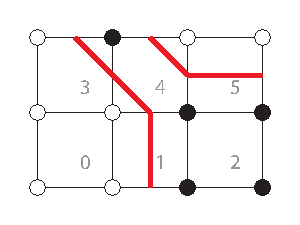
\includegraphics{images/ExampleMesh}
  \caption{Mesh for contour algorithm examples.}
  \label{fig:ExampleMesh}
  \vspace{-2\baselineskip}
\end{wrapfigure}

Three very common patterns in scientific visualization are stream
compaction, reverse index lookup, and topology consolidation. In this
section we describe these patterns using a Marching-Square-like algorithm
applied to the simple example mesh shown in Figure~\ref{fig:ExampleMesh}.

\subsection{Stream Compaction}

\noindent
One common feature of visualization algorithms is that the size of the
output might depend on the data values in the input and cannot be
determined without first analyzing the data. For example, in the mesh of
Figure~\ref{fig:ExampleMesh} we note that there is no contour in cells 0
and 2, a single contour line in cells 1, 3, and 5, and two contour lines in
cell 4. When generating these contour segments in parallel, it is not known
where to place the results. We could allocate space assuming the worst case
scenario that every cell has the maximum number of contour segments, but
that guess tends to be much larger than the actual required memory.
Instead, we want to pack the result tightly in an array. This process is
known as \keyterm{stream compaction}. Stream compaction can be performed in
two data parallel operations, which are demonstrated in
Figure~\ref{fig:StreamCompaction} (adapted from Lo, Sewell, and
Ahrens\scite{PISTON}).

\begin{figure}[htb]
  \centering
  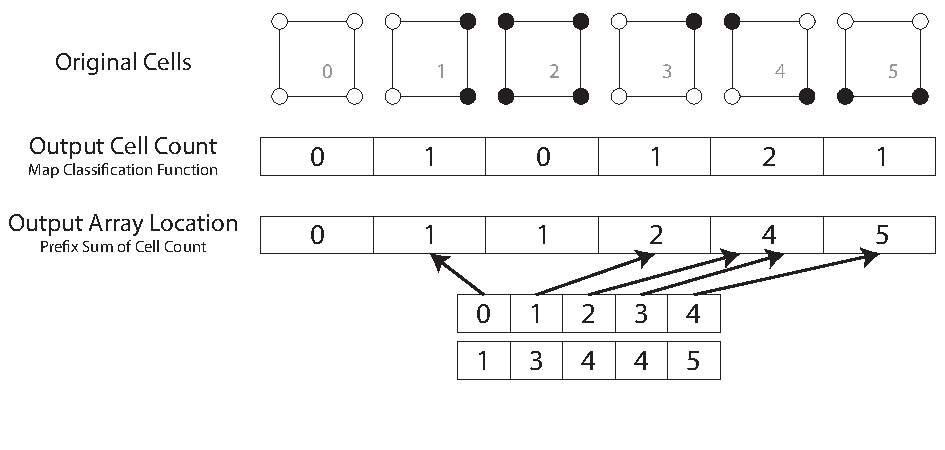
\includegraphics[scale=.9]{images/StreamCompaction}
  \caption{Steps to perform the stream compaction pattern using data
    parallel primitives.}
  \label{fig:StreamCompaction}
\end{figure}

First, a mapping operation is performed to count the size of the output per
cell. Second, an exclusive prefix sum (scan) operation is performed. The
result of the prefix sum for each entry is the sum of all output up to
that point. This sum can be directly used as an index into the compact
output array. A final map of the per-element algorithm can now run, placing
its results into the appropriate location of the output array.

\subsection{Reverse Index Lookup}

\noindent
Directly using the indices from the stream compaction operation results in
a \keyterm{scatter} operation where each thread takes data from an input
element and writes to one or more output elements using random access.
Although the scatter done by the basic stream compaction is functionally
correct, it is known that current many-core processors tend to perform
better with \keyterm{gather} operations where each thread is assigned a
single output element but can access random input
elements\lcite{Stratton2012}. The steps to reverse the index lookup from a
scatter to a gather are demonstrated in Figure~\ref{fig:ReverseLookup}.

\begin{figure}[htb]
  \centering
  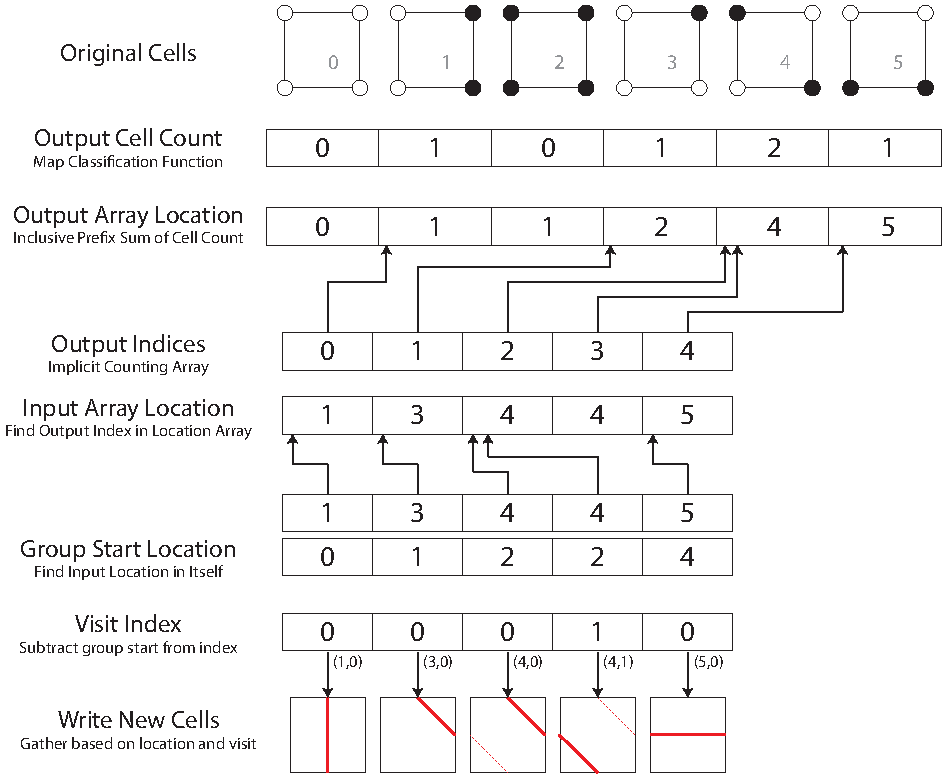
\includegraphics[scale=.9]{images/ReverseLookup}
  \caption{Steps to perform a reverse lookup after stream compaction using
    data parallel primitives.}
  \label{fig:ReverseLookup}
\end{figure}

We start with an array that maps each input to the location in its
corresponding output location. However, we generate this output array
location using an inclusive scan rather than an exclusive scan. This has
the effect of shifting the array to the left by one to make the indexing of
the next step work better. The next step is to search for the upper bound
of the array location for each output element index. The upper bound will
be the first entry greater than the value we search for. This search
requires the target array location indices to be sorted, which it assuredly
is because it is generated from a prefix sum. The search for every index
can be done independently in parallel.

The results from the upper bound give the reverse map from output index
to input index. However, a problem that arises is that multiple output
elements may come from the same input elements but are expected to produce
unique results. In this example input cell 4 produces two contour
elements, so two entries in the input array location map point to that
cell. How are the threads running on these two cells to know which element
to produce? We solve this problem by generating what we call a
\keyterm{visit index}.

The visit indices are generated in two steps. First, we perform a lower
bound search of each value in the input array location map into the same
map. The lower bound search finds the last entry less than or equal to the
value we search for in
parallel. The result is the index to the first entry in the input array
location map for the group associated with the same input element. We then
take this array of indices and subtract them from the output index to get a
unique index into that group. We call this the visit index. Using the pair
from input array location map and the visit index, each thread running for
a single output element can uniquely generate the data it is to produce.

\subsection{Topology Consolidation}

\noindent
Another common occurrence in visualization algorithms is for independent
threads to redundantly create coincident data. For example, output elements
0 and 3 from Figures \ref{fig:StreamCompaction} and \ref{fig:ReverseLookup}
come from cells 1 and 4, respectively, in Figure~\ref{fig:ExampleMesh} and
share a vertex. This shared vertex is independently interpolated in
separate threads and the connection of these output elements is lost. It is
sometimes required to consolidate the topology by finding these coincident
elements and merging them.

The general approach to topology consolidation is to define a simple hash
for each element that uniquely identifies the element for all instances.
That is, two hash values are equal if and only if the associated elements
are coincident. Once hashes are generated, a sort keyed on the hashes moves
all coincident elements to be adjacent in the storage arrays. At this point
it is straightforward to designate groups of coincident
elements and reduce the groups to a single element in parallel.

For the specific case of merging vertices, Bell\scite{Bell2010} proposes
using the point coordinate triple as the hash. However, that approach is
intolerant to any numerical inaccuracy. A better approach is to use
integer-based hashes, which can usually be derived from the input topology.
For example, contour algorithms like Marching Cubes always define contour
vertices on the edges of the input mesh. These edges (and therefore the
vertices) can be uniquely defined either by an enumerated index or by the
pair of indices for the edge's vertex endpoints. Miller, Moreland, and
Ma\scite{Miller2014} show this approach is faster than using point
coordinates and can also be applied to topological elements other than
vertices.


\section{Results}

\noindent
One of the promises of using data parallel primitives to build scientific
visualization algorithms is performance portability. That is, a single
implementation using data parallel primitives should work well across
computing devices with vastly different performance characteristics from
traditional latency-optimized multi-core CPUs to bandwidth-optimized
many-core GPUs. Furthermore, portable data parallel primitive
implementations should have close to the performance of a non-portable
algorithm designed and optimized specifically for a particular device.
Recent research indicates that data parallel primitive algorithms are in
fact quite performance portable.

Maynard \etal\scite{Maynard2013} compare a threshold algorithm written with
data parallel primitives across many devices. The algorithm shows good
performance on both multi-core CPU and many-core GPU devices.
Interestingly, the data parallel primitive algorithm running serially on a
single CPU core still beats the equivalent VTK implementation.

Lo, Sewell, and Ahrens\scite{PISTON} demonstrate the performance of a
Marching Cubes algorithm implemented with data parallel primitives. Their
algorithm is compared with the equivalent CUDA reference implementation
optimized for that architecture. The two implementations get comparable
performance. The data parallel primitive implementation is also shown to
get good performance and scalability on multi-core CPUs.

But perhaps the most encouraging evidence comes from a recent performance
study conducted by Larsen \etal\scite{Larsen:PacVis2015} for ray tracing in
the context of data parallel primitives.
%
Ray tracing is a challenging use case since it is computationally
intense and contains both regular and irregular memory access patterns.
%
Moreover, this is an algorithm with ``guaranteed not to exceed''
standards, in the form of Intel's Embree\scite{wald2014embree} and
NVIDIA's OptiX\scite{parker2010optix}.
%
These products each are supported by teams of developers and have been under
development for multiple years. 
%
Further, they make full use of architectural knowledge, including
constructs like intrinsics, and tune for
Intel and NVIDIA products, respectively.

\begin{wrapfigure}{R}{2.64in}
  %\vspace{-\baselineskip}
  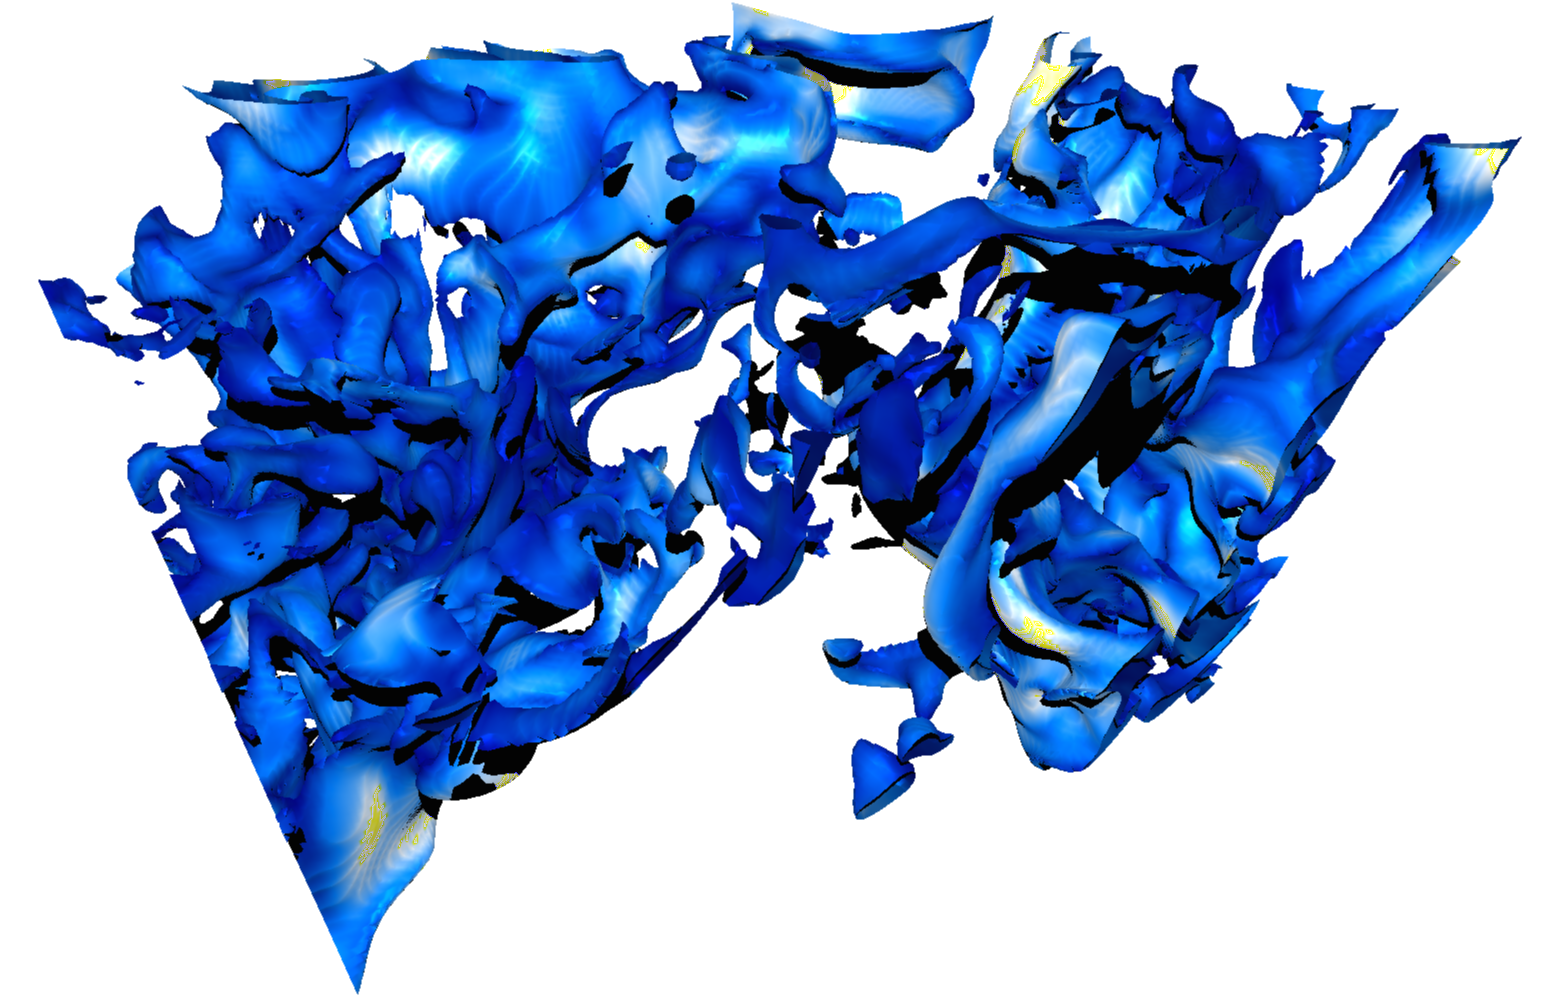
\includegraphics[width=2.64in]{images/rm650_teaser}
  \caption{Rendering from ray tracing study on an isosurface of 650,000 triangles.\\}
  \label{fig:raytracing}
  \vspace{-\baselineskip}
\end{wrapfigure}
Larsen implements his ray tracer within EAVL and provides a performance
study against OptiX on multiple NVIDIA GPUs and against Embree on Intel Xeon
and Xeon Phi architectures.  
%
His study includes both scientific data sets and standard
ray tracing data sets (e.g., Stanford dragon).
%
Figure~\ref{fig:raytracing} shows one of the scientific data sets.

Encouragingly, the performance comparison finds that the EAVL
ray tracer is competitive with the industry standards.
%
It is within a factor of two on most configurations and does particularly
well on the scientific data sets.
%
In fact, it even outperforms the industry standards on some older
architectures (since the industry standards tend to focus on 
the latest architectures).
%

Overall, this result is encouraging regarding the prospects for portable
performance with data parallel primitives, in that 
a single, architecture-agnostic implementation was comparable to two 
highly-tuned, architecture-specific standards.
%
Although the architecture-specific standards are clearly faster, the gap
is likely acceptable for our use case.
%
Further, the data parallel primitive approach is completed by a graduate
student in a period of months whereas the industry standards take
experts years (or more); the encumbrence from data parallel
primitives could actually be even smaller given additional effort and expertise.

\section{Conclusion}

\noindent
Visualization software will need significant changes to excel in
the exascale era, both to deal with diverse architectures and to 
deal with massive concurrency within a node.
%
Recent results show that data parallel primitives are a promising technology
to deal with both challenges.
%
First, exploration into multiple algorithms have shown recurring
trends, and will hopefully serve as a precursor to porting many of our
community's algorithms reusing these same trends.
%
Second, studies comparing performance with architecture-specific
implementations have shown that the performance is very good.
%
Researchers in this area --- including the authors of this paper ---
are so encouraged that they have banded together to form a new effort, 
VTK-m, in an endeavor to provide production visualization software
to the HPC community.

\ack{
  This material is based upon work supported by the U.S. Department of
  Energy, Office of Science, Office of Advanced Scientific Computing
  Research, under Award Numbers 10-014707, 12-015215, and 14-017566.

  Sandia National Laboratories is a multi-program laboratory managed and
  operated by Sandia Corporation, a wholly owned subsidiary of Lockheed
  Martin Corporation, for the U.S. Department of Energy's National Nuclear
  Security Administration under contract DE-AC04-94AL85000.
}

{\scriptsize SAND 2015-2273 C}


\bibliographystyle{plain}
\bibliography{SCFrontiers2015}

\end{document}
